\documentclass[10pt]{article}
\usepackage[margin=0.65in]{geometry}
\usepackage{graphicx}
\usepackage{booktabs}
\usepackage{longtable}
\usepackage{float}
\begin{document}
\title{GEOS-MPM Validation Suite Report}
\author{Generated by validation/runValidationSuite}
\date{May 17, 2026}
\maketitle
\section*{Running and rerunning}
Cases are staged under \texttt{testRunDirectory/validation/<case>}. The suite records failures and continues unless \texttt{--stop-on-error} is supplied.
\begin{verbatim}
cd scripts/preProcessing/materialPointMethodParticleFileWriter/validation
./runValidationSuite all --python /usr/tce/bin/python3 --force
./runValidationSuite report --python /usr/tce/bin/python3
\end{verbatim}
\section*{Timing and dispatch summary}
\small
\begin{longtable}{p{0.27\linewidth}p{0.13\linewidth}p{0.18\linewidth}p{0.11\linewidth}p{0.14\linewidth}p{0.09\linewidth}p{0.09\linewidth}}
\toprule Case & Status & Family & GEOS job & GEOS state & GEOS wall & Post wall \\ \midrule\endhead
geomechanics\_\_geoOHCrD\_2024\_ISR08\_V5 & not run & Geomechanics &  &  &  &  \\
geomechanics\_\_geomechanicsHydrostaticCreep\_HP03 & not run & Geomechanics &  &  &  &  \\
geomechanics\_\_geomechanicsTriaxialCompression\_ISR03 & not run & Geomechanics &  &  &  &  \\
geomechanics\_\_geomechanicsTriaxialCompression\_TP1 & not run & Geomechanics &  &  &  &  \\
geomechanics\_\_geomechanicsTriaxialCompression\_TP2 & not run & Geomechanics &  &  &  &  \\
geomechanics\_\_geomechanicsTriaxialCompression\_TP3 & not run & Geomechanics &  &  &  &  \\
geomechanics\_\_geomechanicsTriaxialCreep\_TC02 & not run & Geomechanics &  &  &  &  \\
polymer\_\_polymerCompression & submitted & Polymer validation & 6046423 & COMPLETED & 00:00:29 & 00:00:16 \\
polymer\_\_polymerTension & submitted & Polymer validation & 6046425 & COMPLETED & 00:00:34 & 00:00:16 \\
\bottomrule
\end{longtable}
\normalsize
\clearpage
\section*{geomechanics / geoOHCrD 2024 ISR08 V5}
Validation case for Geomechanics.
\begin{figure}[H]\centering
\includegraphics[width=0.58\linewidth]{schematics/geomechanics\_\_geoOHCrD\_2024\_ISR08\_V5\_schematic.png}
\caption{Schematic for geomechanics\_\_geoOHCrD\_2024\_ISR08\_V5.}
\end{figure}
\textbf{Code features exercised.}
\begin{itemize}
\item reaction-history output
\item box-average history
\item Geomechanics constitutive model
\item temperature table/event
\end{itemize}
\begin{figure}[H]\centering
\fbox{\begin{minipage}[c][1.15in][c]{0.29\linewidth}\centering missing initial\end{minipage}}
\fbox{\begin{minipage}[c][1.15in][c]{0.29\linewidth}\centering missing final\end{minipage}}
\fbox{\begin{minipage}[c][1.15in][c]{0.29\linewidth}\centering missing history/comparison\end{minipage}}
\caption{Initial state, final state, and history/comparison plot for geomechanics\_\_geoOHCrD\_2024\_ISR08\_V5.}
\end{figure}
\paragraph{Reference or legacy comparison assets.}
\begin{figure}[H]\centering
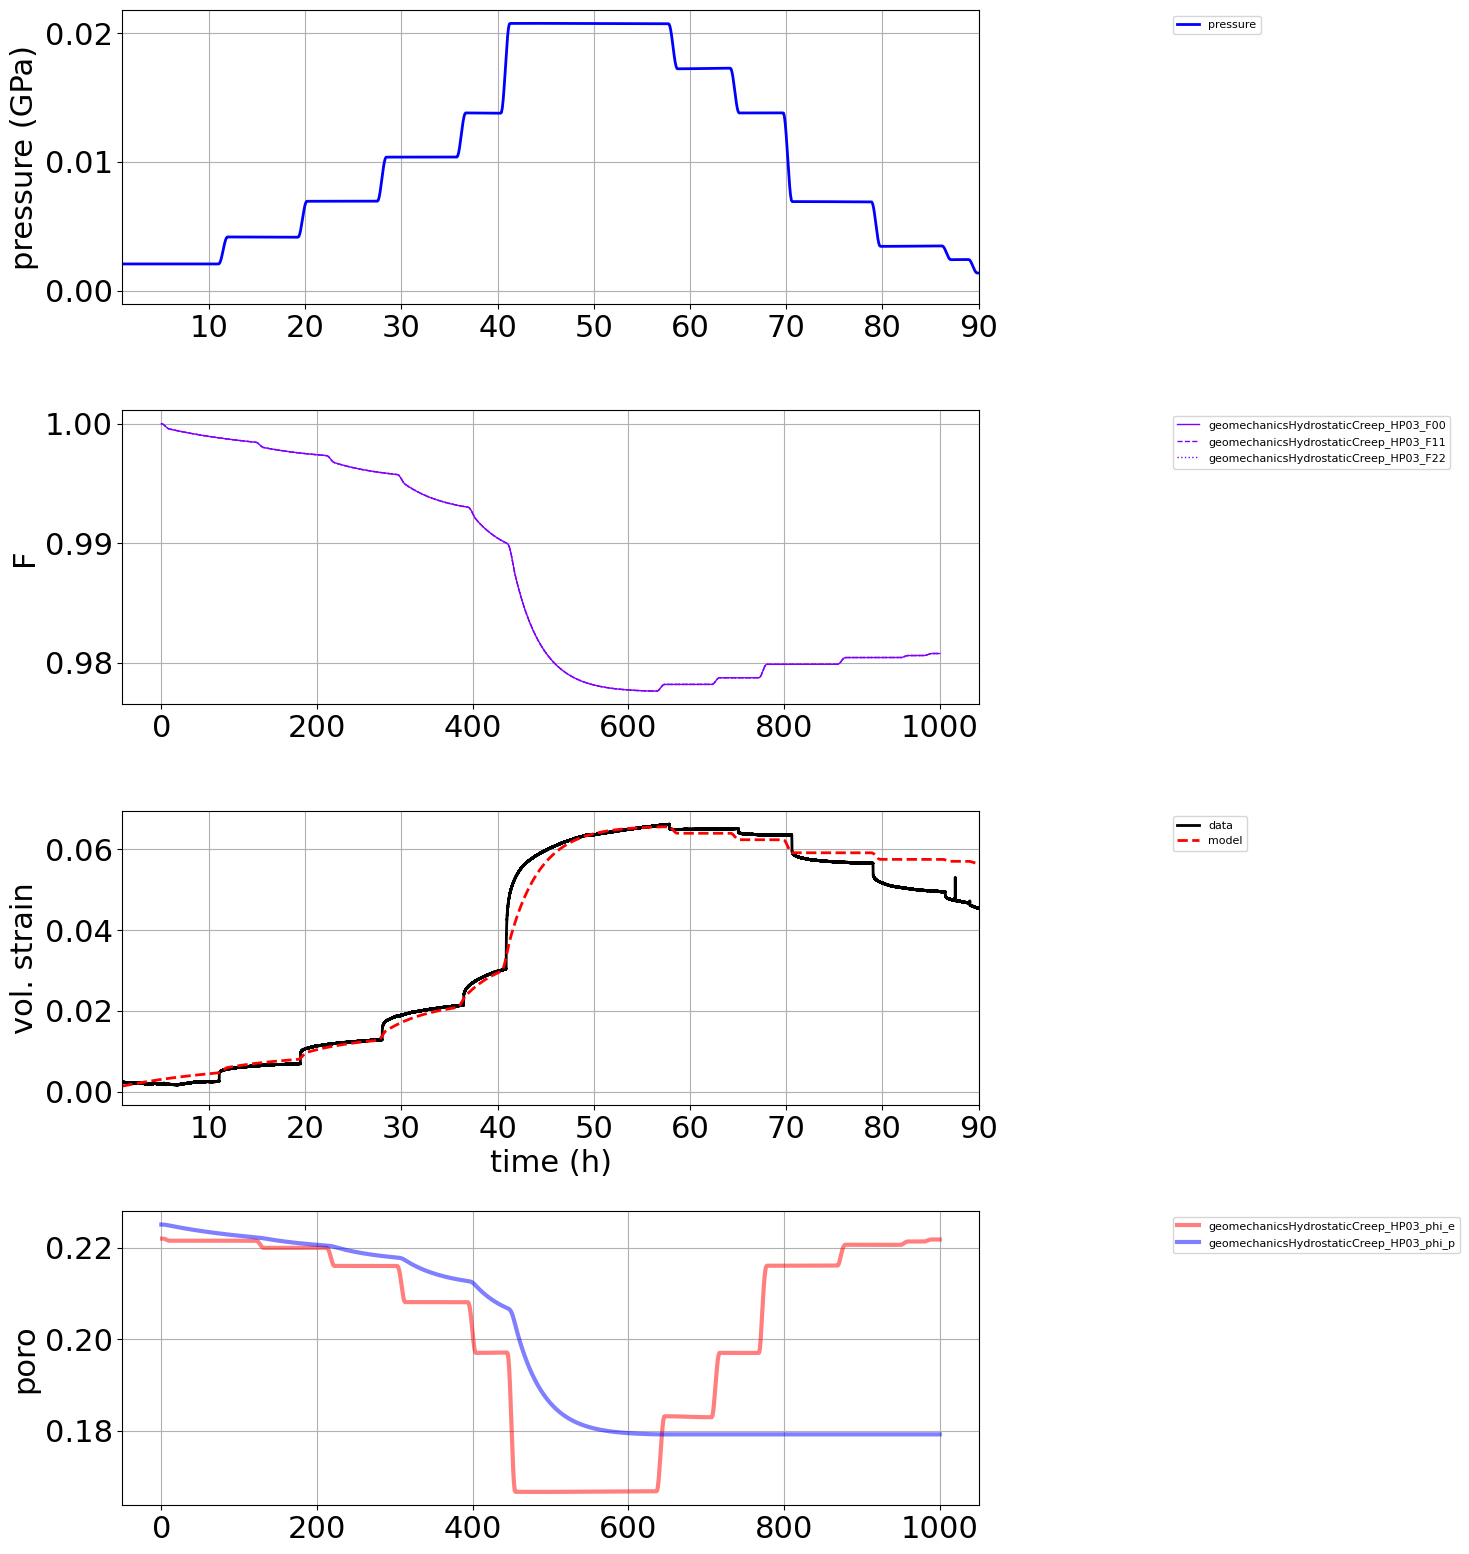
\includegraphics[width=0.42\linewidth]{../geomechanics/geomechanicsHydrostaticCreep.png}
\includegraphics[width=0.42\linewidth]{../geomechanics/geomechanicsTriaxialCompression\_ISR03.png}
\caption{Existing comparison assets in the source case directory.}
\end{figure}
\clearpage
\section*{geomechanics / geomechanicsHydrostaticCreep HP03}
Validation case for Geomechanics.
\begin{figure}[H]\centering
\includegraphics[width=0.58\linewidth]{schematics/geomechanics\_\_geomechanicsHydrostaticCreep\_HP03\_schematic.png}
\caption{Schematic for geomechanics\_\_geomechanicsHydrostaticCreep\_HP03.}
\end{figure}
\textbf{Code features exercised.}
\begin{itemize}
\item reaction-history output
\item box-average history
\item Geomechanics constitutive model
\item VonMisesJ plasticity
\end{itemize}
\begin{figure}[H]\centering
\fbox{\begin{minipage}[c][1.15in][c]{0.29\linewidth}\centering missing initial\end{minipage}}
\fbox{\begin{minipage}[c][1.15in][c]{0.29\linewidth}\centering missing final\end{minipage}}
\fbox{\begin{minipage}[c][1.15in][c]{0.29\linewidth}\centering missing history/comparison\end{minipage}}
\caption{Initial state, final state, and history/comparison plot for geomechanics\_\_geomechanicsHydrostaticCreep\_HP03.}
\end{figure}
\paragraph{Reference or legacy comparison assets.}
\begin{figure}[H]\centering
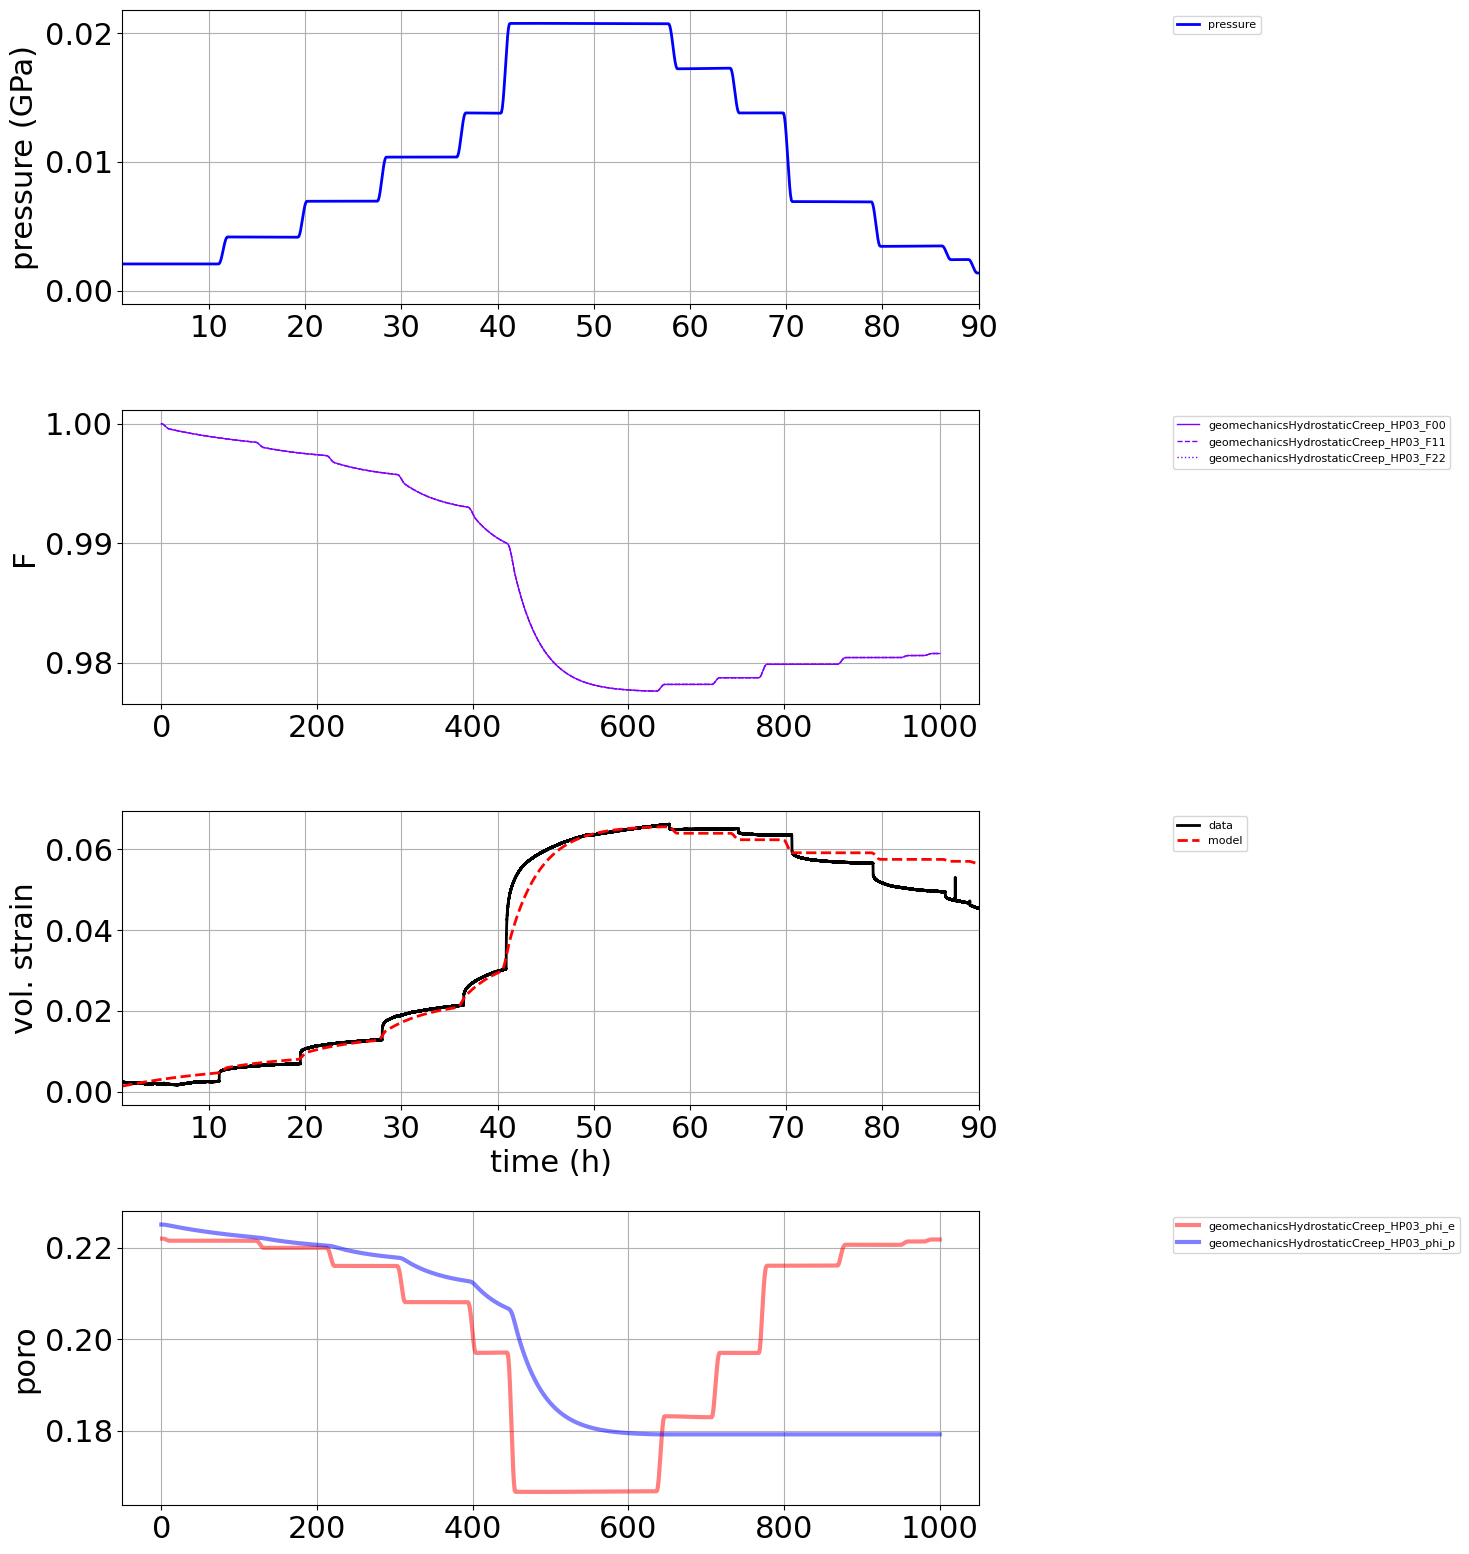
\includegraphics[width=0.42\linewidth]{../geomechanics/geomechanicsHydrostaticCreep.png}
\includegraphics[width=0.42\linewidth]{../geomechanics/geomechanicsTriaxialCompression\_ISR03.png}
\caption{Existing comparison assets in the source case directory.}
\end{figure}
\clearpage
\section*{geomechanics / geomechanicsTriaxialCompression ISR03}
Validation case for Geomechanics.
\begin{figure}[H]\centering
\includegraphics[width=0.58\linewidth]{schematics/geomechanics\_\_geomechanicsTriaxialCompression\_ISR03\_schematic.png}
\caption{Schematic for geomechanics\_\_geomechanicsTriaxialCompression\_ISR03.}
\end{figure}
\textbf{Code features exercised.}
\begin{itemize}
\item FMPM update
\item XPIC/PIC-family transfer
\item reaction-history output
\item box-average history
\item Geomechanics constitutive model
\end{itemize}
\begin{figure}[H]\centering
\fbox{\begin{minipage}[c][1.15in][c]{0.29\linewidth}\centering missing initial\end{minipage}}
\fbox{\begin{minipage}[c][1.15in][c]{0.29\linewidth}\centering missing final\end{minipage}}
\fbox{\begin{minipage}[c][1.15in][c]{0.29\linewidth}\centering missing history/comparison\end{minipage}}
\caption{Initial state, final state, and history/comparison plot for geomechanics\_\_geomechanicsTriaxialCompression\_ISR03.}
\end{figure}
\paragraph{Reference or legacy comparison assets.}
\begin{figure}[H]\centering
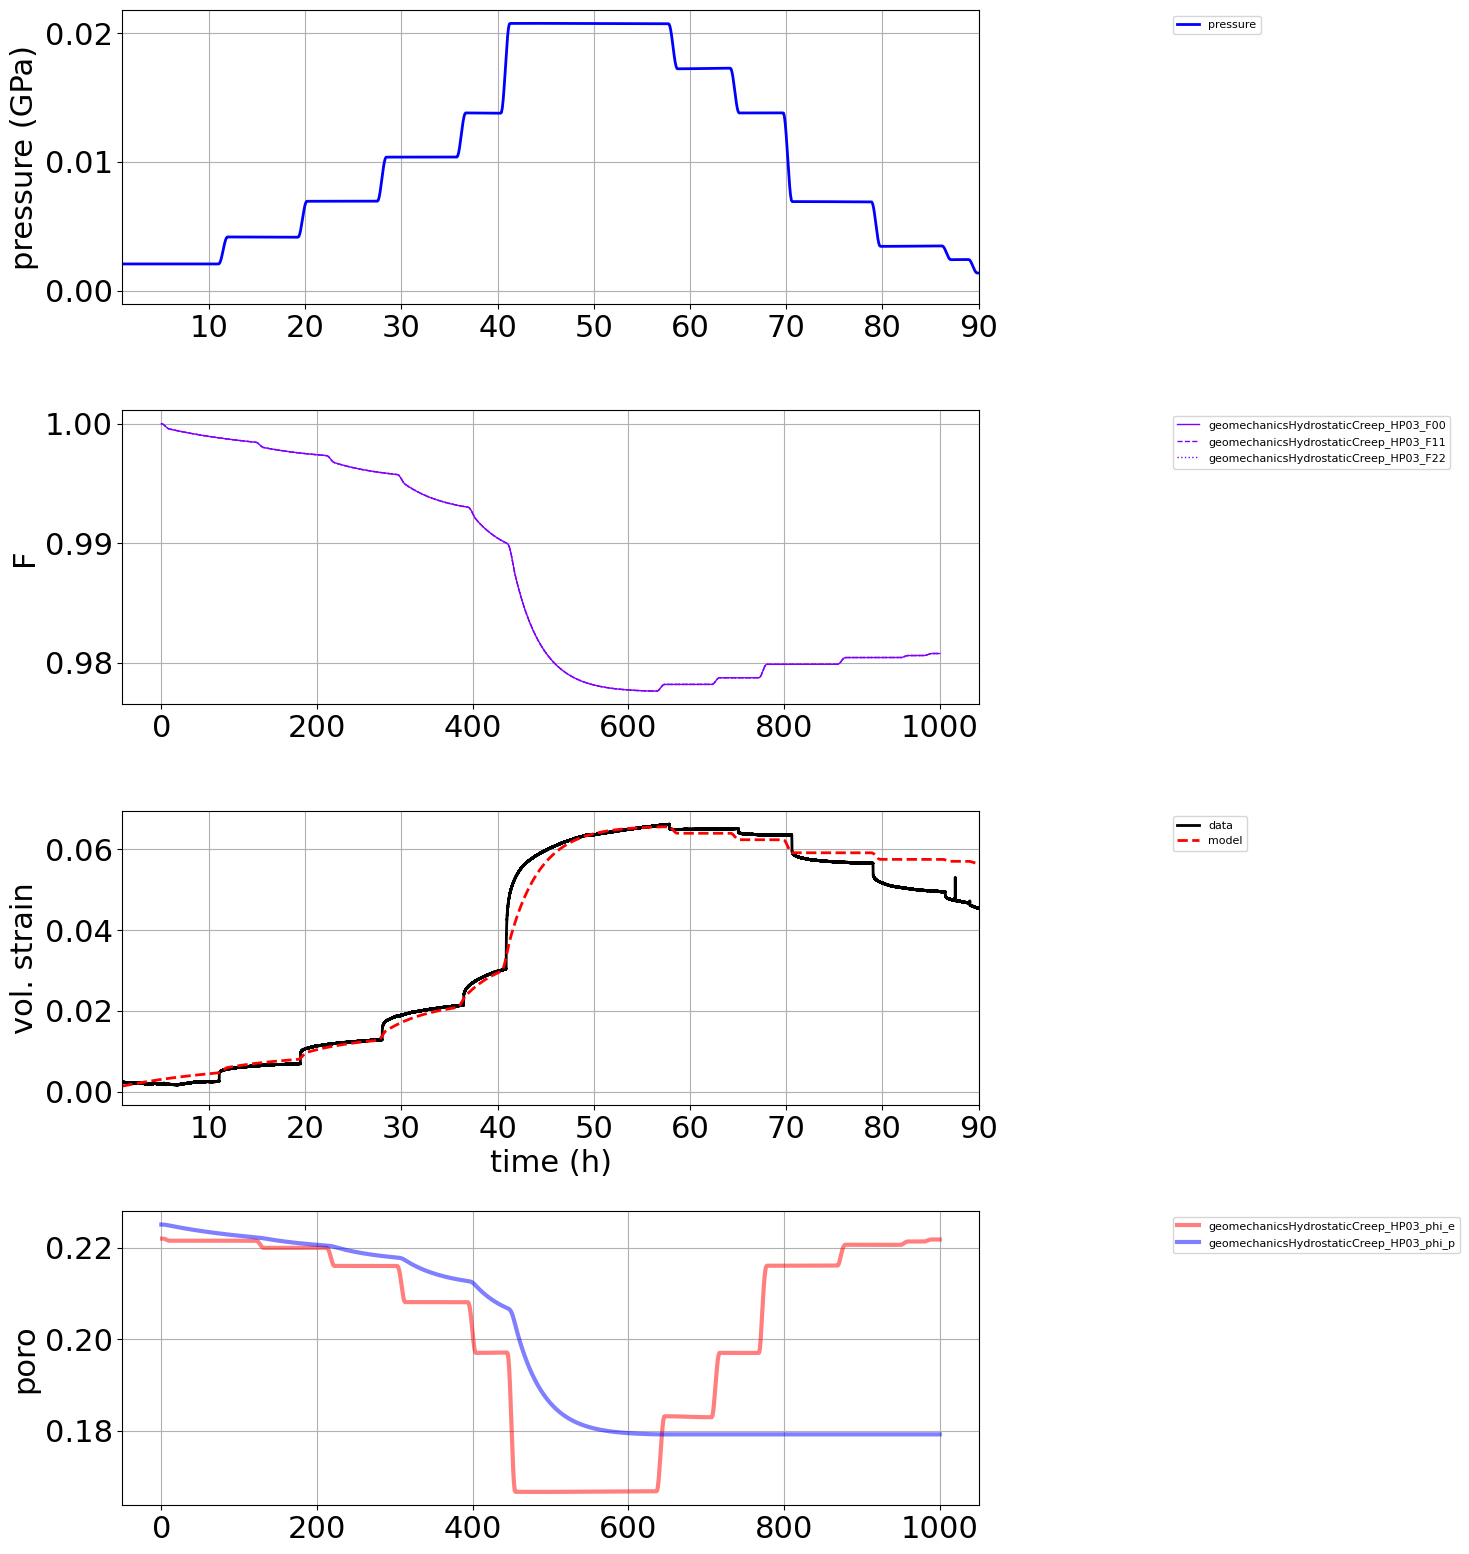
\includegraphics[width=0.42\linewidth]{../geomechanics/geomechanicsHydrostaticCreep.png}
\includegraphics[width=0.42\linewidth]{../geomechanics/geomechanicsTriaxialCompression\_ISR03.png}
\caption{Existing comparison assets in the source case directory.}
\end{figure}
\clearpage
\section*{geomechanics / geomechanicsTriaxialCompression TP1}
Validation case for Geomechanics.
\begin{figure}[H]\centering
\includegraphics[width=0.58\linewidth]{schematics/geomechanics\_\_geomechanicsTriaxialCompression\_TP1\_schematic.png}
\caption{Schematic for geomechanics\_\_geomechanicsTriaxialCompression\_TP1.}
\end{figure}
\textbf{Code features exercised.}
\begin{itemize}
\item FMPM update
\item XPIC/PIC-family transfer
\item reaction-history output
\item box-average history
\item Geomechanics constitutive model
\end{itemize}
\begin{figure}[H]\centering
\fbox{\begin{minipage}[c][1.15in][c]{0.29\linewidth}\centering missing initial\end{minipage}}
\fbox{\begin{minipage}[c][1.15in][c]{0.29\linewidth}\centering missing final\end{minipage}}
\fbox{\begin{minipage}[c][1.15in][c]{0.29\linewidth}\centering missing history/comparison\end{minipage}}
\caption{Initial state, final state, and history/comparison plot for geomechanics\_\_geomechanicsTriaxialCompression\_TP1.}
\end{figure}
\paragraph{Reference or legacy comparison assets.}
\begin{figure}[H]\centering
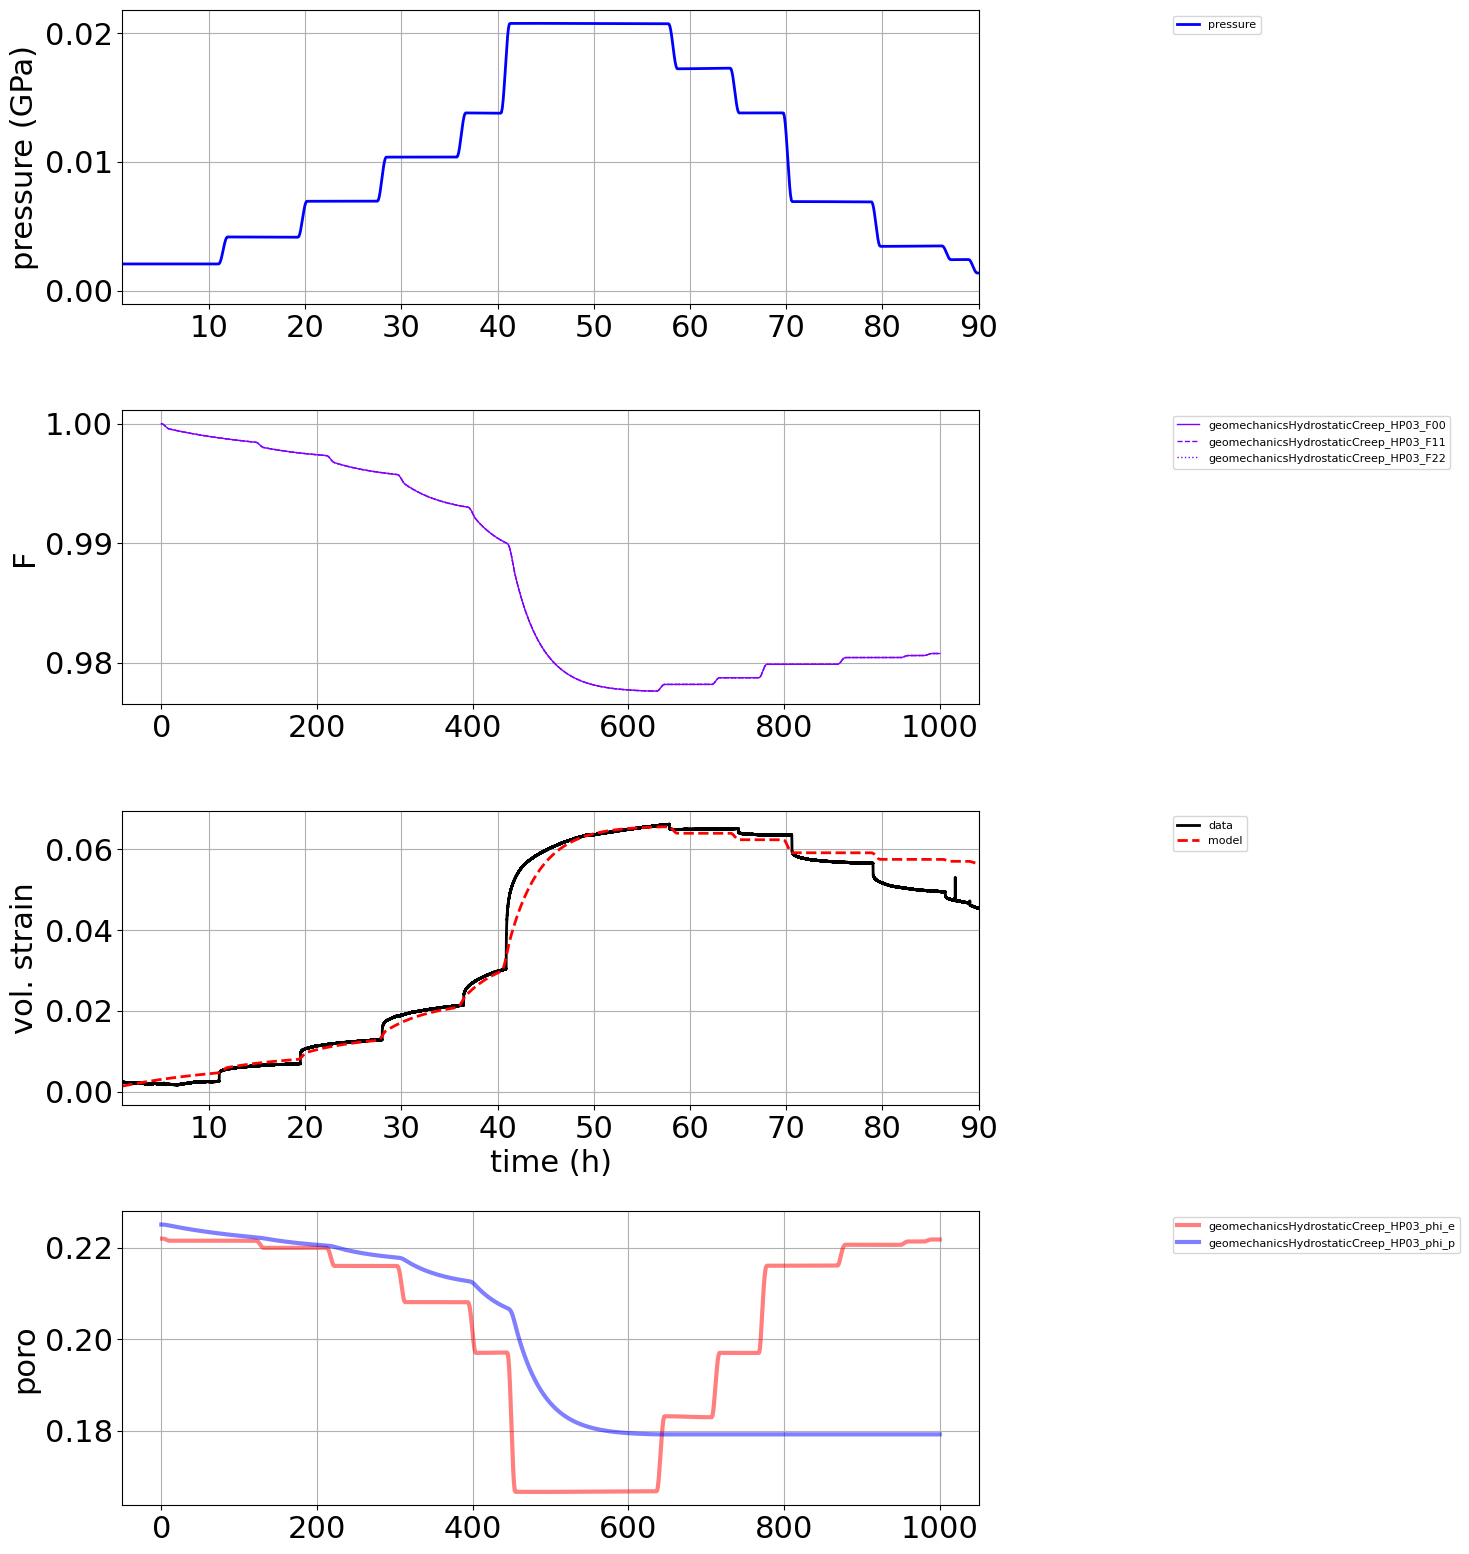
\includegraphics[width=0.42\linewidth]{../geomechanics/geomechanicsHydrostaticCreep.png}
\includegraphics[width=0.42\linewidth]{../geomechanics/geomechanicsTriaxialCompression\_ISR03.png}
\caption{Existing comparison assets in the source case directory.}
\end{figure}
\clearpage
\section*{geomechanics / geomechanicsTriaxialCompression TP2}
Validation case for Geomechanics.
\begin{figure}[H]\centering
\includegraphics[width=0.58\linewidth]{schematics/geomechanics\_\_geomechanicsTriaxialCompression\_TP2\_schematic.png}
\caption{Schematic for geomechanics\_\_geomechanicsTriaxialCompression\_TP2.}
\end{figure}
\textbf{Code features exercised.}
\begin{itemize}
\item FMPM update
\item XPIC/PIC-family transfer
\item reaction-history output
\item box-average history
\item Geomechanics constitutive model
\end{itemize}
\begin{figure}[H]\centering
\fbox{\begin{minipage}[c][1.15in][c]{0.29\linewidth}\centering missing initial\end{minipage}}
\fbox{\begin{minipage}[c][1.15in][c]{0.29\linewidth}\centering missing final\end{minipage}}
\fbox{\begin{minipage}[c][1.15in][c]{0.29\linewidth}\centering missing history/comparison\end{minipage}}
\caption{Initial state, final state, and history/comparison plot for geomechanics\_\_geomechanicsTriaxialCompression\_TP2.}
\end{figure}
\paragraph{Reference or legacy comparison assets.}
\begin{figure}[H]\centering
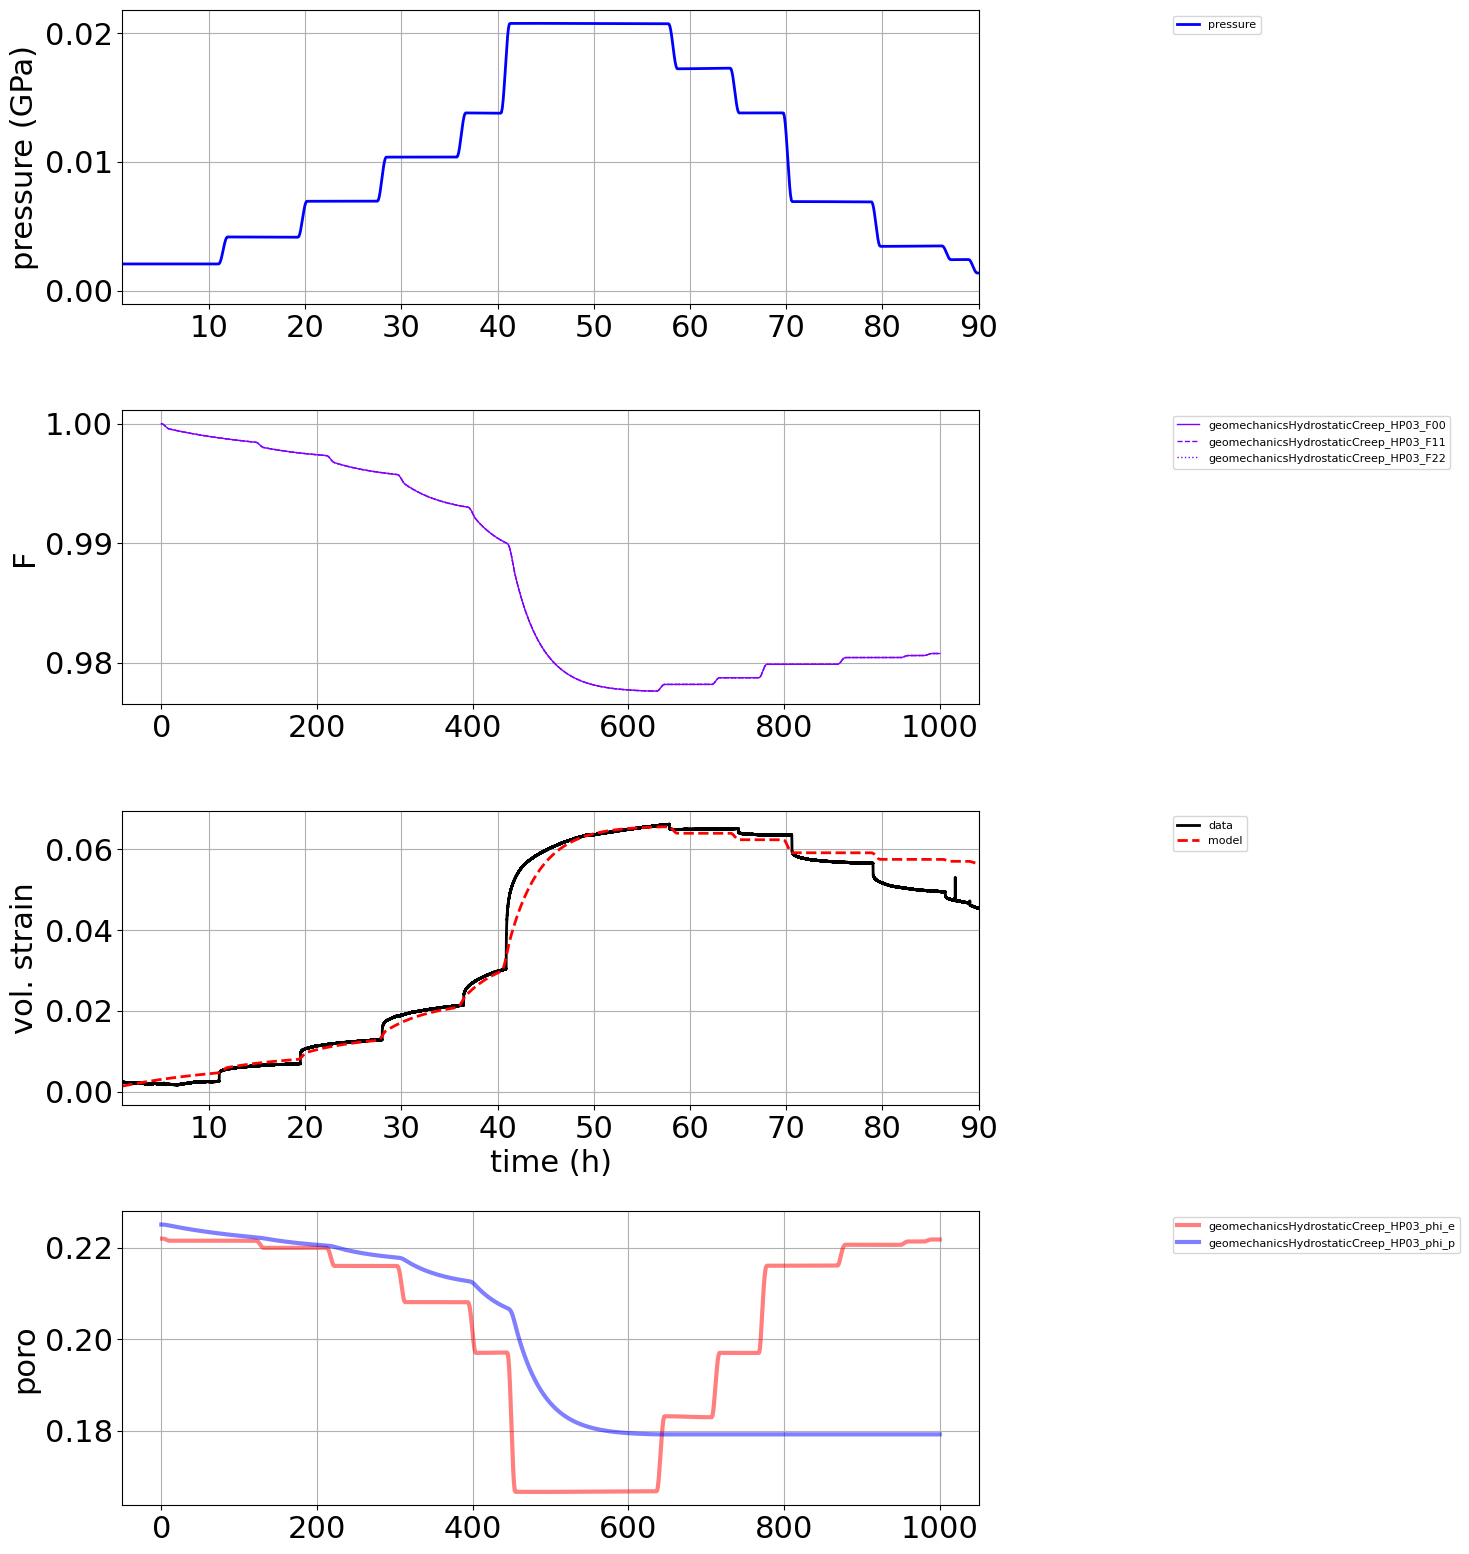
\includegraphics[width=0.42\linewidth]{../geomechanics/geomechanicsHydrostaticCreep.png}
\includegraphics[width=0.42\linewidth]{../geomechanics/geomechanicsTriaxialCompression\_ISR03.png}
\caption{Existing comparison assets in the source case directory.}
\end{figure}
\clearpage
\section*{geomechanics / geomechanicsTriaxialCompression TP3}
Validation case for Geomechanics.
\begin{figure}[H]\centering
\includegraphics[width=0.58\linewidth]{schematics/geomechanics\_\_geomechanicsTriaxialCompression\_TP3\_schematic.png}
\caption{Schematic for geomechanics\_\_geomechanicsTriaxialCompression\_TP3.}
\end{figure}
\textbf{Code features exercised.}
\begin{itemize}
\item FMPM update
\item XPIC/PIC-family transfer
\item reaction-history output
\item box-average history
\item Geomechanics constitutive model
\end{itemize}
\begin{figure}[H]\centering
\fbox{\begin{minipage}[c][1.15in][c]{0.29\linewidth}\centering missing initial\end{minipage}}
\fbox{\begin{minipage}[c][1.15in][c]{0.29\linewidth}\centering missing final\end{minipage}}
\fbox{\begin{minipage}[c][1.15in][c]{0.29\linewidth}\centering missing history/comparison\end{minipage}}
\caption{Initial state, final state, and history/comparison plot for geomechanics\_\_geomechanicsTriaxialCompression\_TP3.}
\end{figure}
\paragraph{Reference or legacy comparison assets.}
\begin{figure}[H]\centering
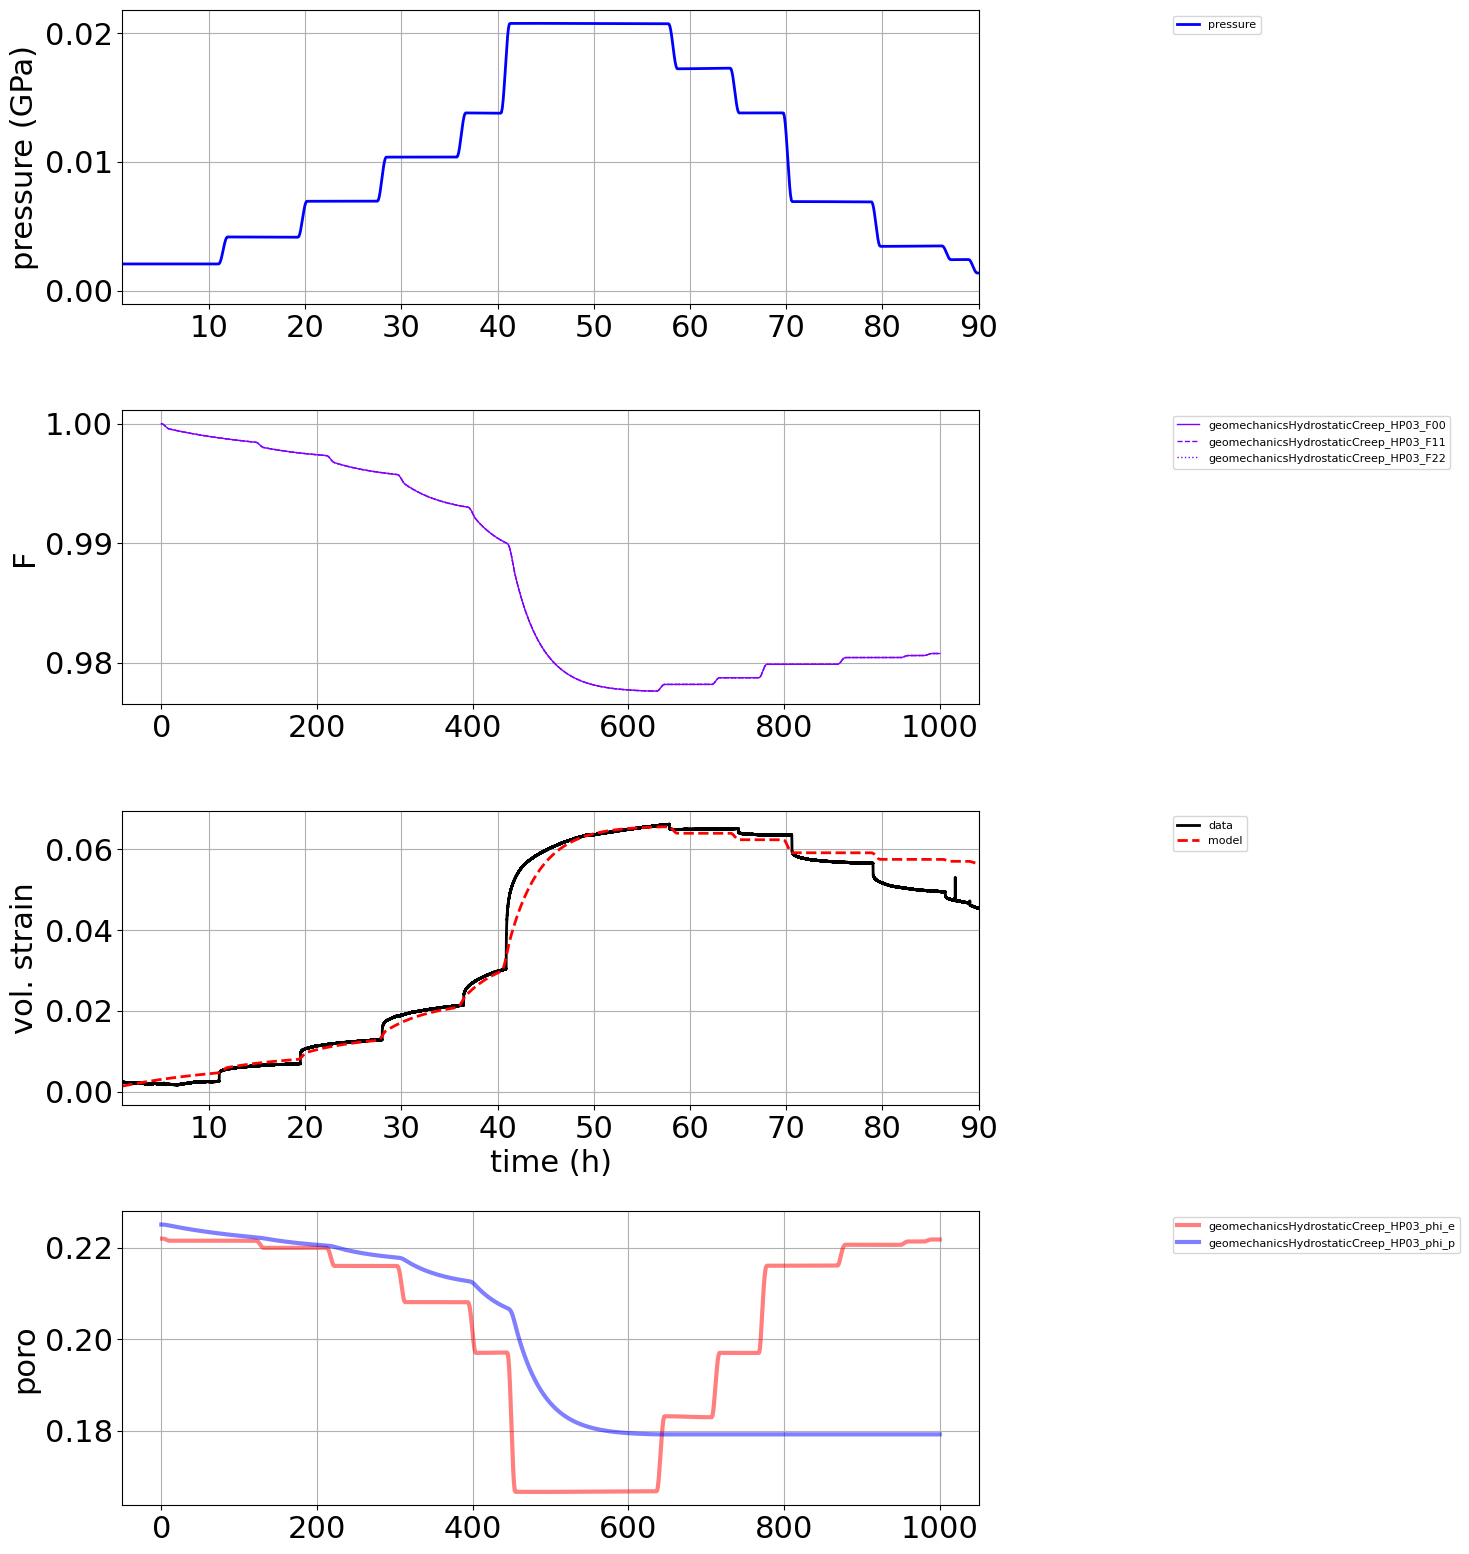
\includegraphics[width=0.42\linewidth]{../geomechanics/geomechanicsHydrostaticCreep.png}
\includegraphics[width=0.42\linewidth]{../geomechanics/geomechanicsTriaxialCompression\_ISR03.png}
\caption{Existing comparison assets in the source case directory.}
\end{figure}
\clearpage
\section*{geomechanics / geomechanicsTriaxialCreep TC02}
Validation case for Geomechanics.
\begin{figure}[H]\centering
\includegraphics[width=0.58\linewidth]{schematics/geomechanics\_\_geomechanicsTriaxialCreep\_TC02\_schematic.png}
\caption{Schematic for geomechanics\_\_geomechanicsTriaxialCreep\_TC02.}
\end{figure}
\textbf{Code features exercised.}
\begin{itemize}
\item FMPM update
\item XPIC/PIC-family transfer
\item reaction-history output
\item box-average history
\item Geomechanics constitutive model
\item VonMisesJ plasticity
\end{itemize}
\begin{figure}[H]\centering
\fbox{\begin{minipage}[c][1.15in][c]{0.29\linewidth}\centering missing initial\end{minipage}}
\fbox{\begin{minipage}[c][1.15in][c]{0.29\linewidth}\centering missing final\end{minipage}}
\fbox{\begin{minipage}[c][1.15in][c]{0.29\linewidth}\centering missing history/comparison\end{minipage}}
\caption{Initial state, final state, and history/comparison plot for geomechanics\_\_geomechanicsTriaxialCreep\_TC02.}
\end{figure}
\paragraph{Reference or legacy comparison assets.}
\begin{figure}[H]\centering
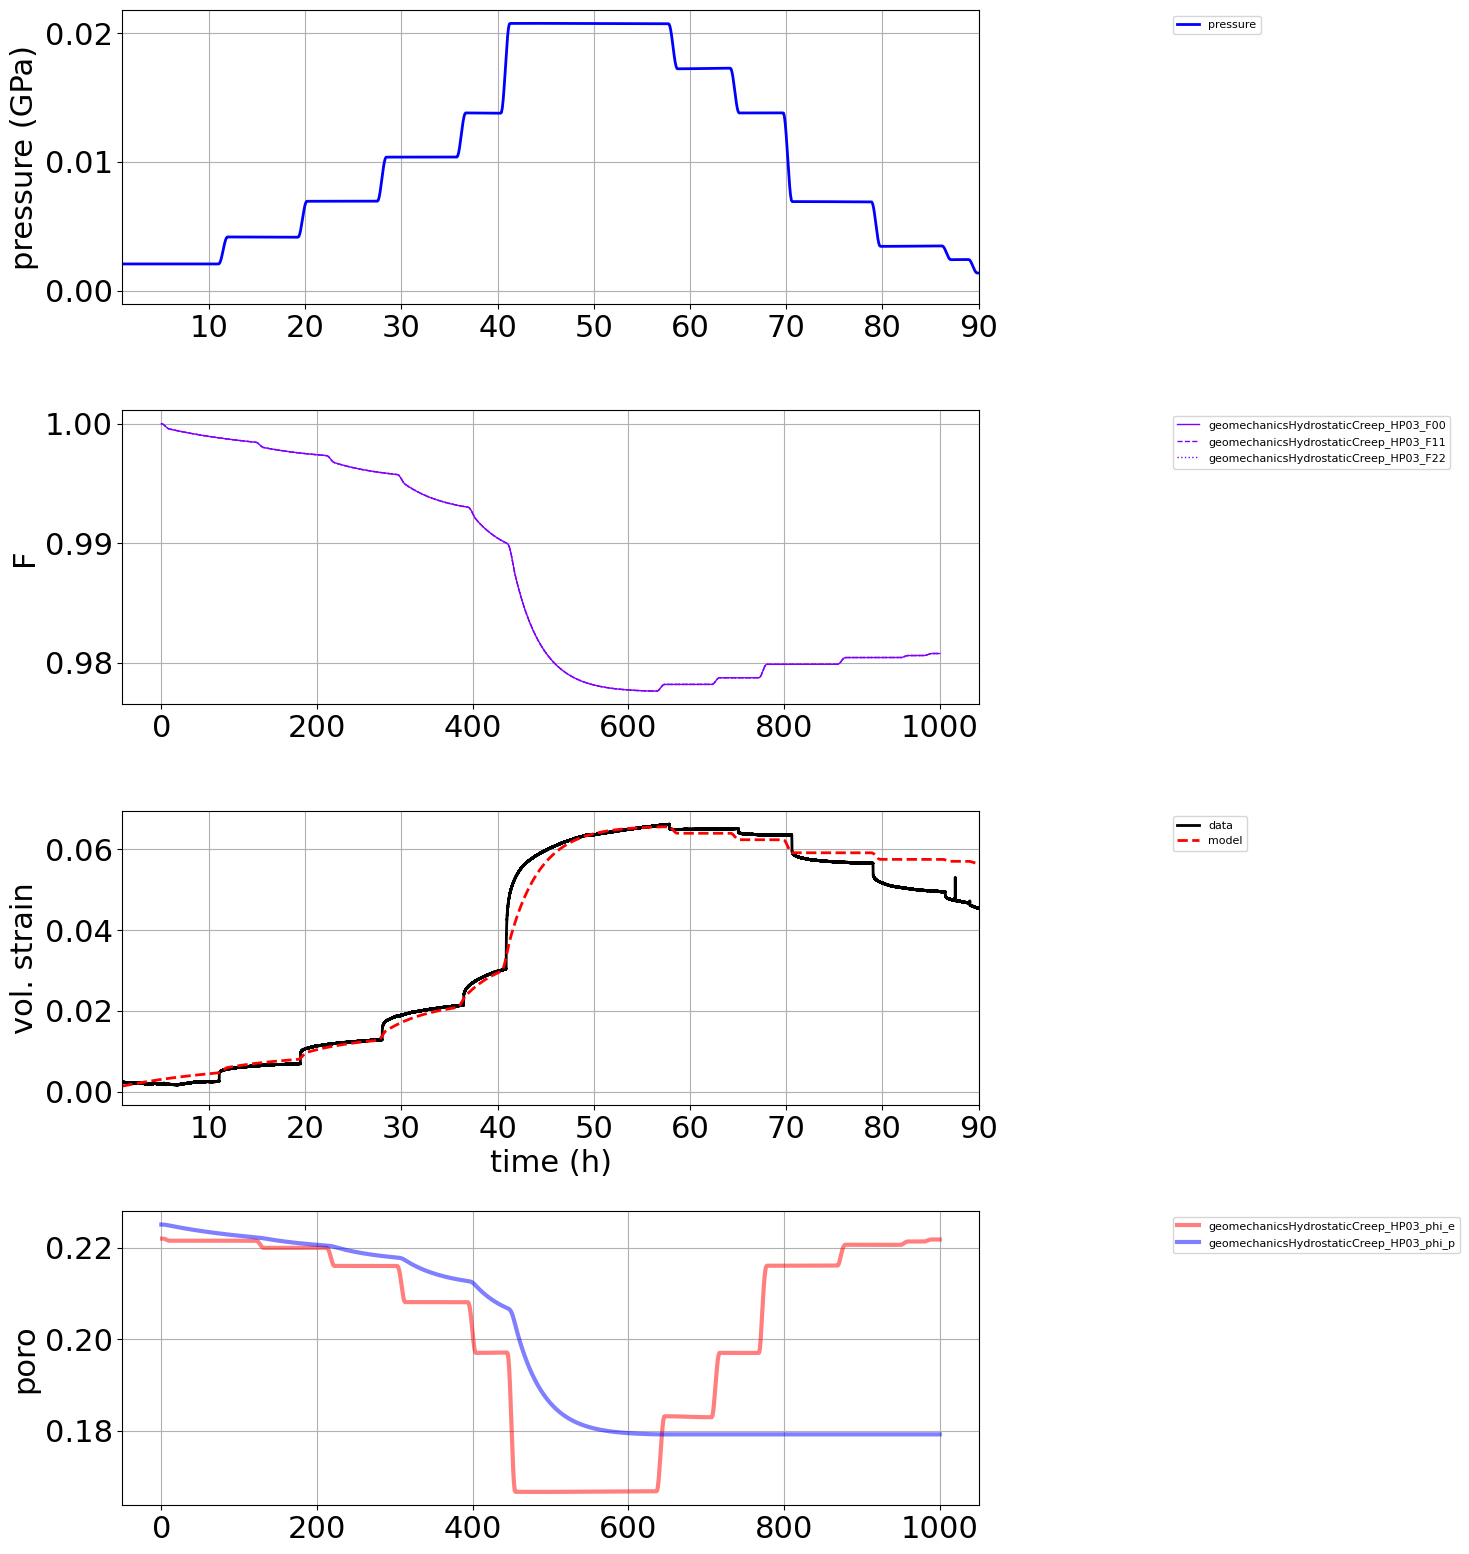
\includegraphics[width=0.42\linewidth]{../geomechanics/geomechanicsHydrostaticCreep.png}
\includegraphics[width=0.42\linewidth]{../geomechanics/geomechanicsTriaxialCompression\_ISR03.png}
\caption{Existing comparison assets in the source case directory.}
\end{figure}
\clearpage
\section*{polymer / polymerCompression}
Validation case for Polymer validation.
\begin{figure}[H]\centering
\includegraphics[width=0.58\linewidth]{schematics/polymer\_\_polymerCompression\_schematic.png}
\caption{Schematic for polymer\_\_polymerCompression.}
\end{figure}
\textbf{Code features exercised.}
\begin{itemize}
\item reaction-history output
\item box-average history
\end{itemize}
\begin{figure}[H]\centering
\includegraphics[width=0.31\linewidth]{../polymer/output/polymer\_\_polymerCompression/polymer\_\_polymerCompression\_initial\_particleStrengthScale.png}
\includegraphics[width=0.31\linewidth]{../polymer/output/polymer\_\_polymerCompression/polymer\_\_polymerCompression\_final\_particleDamage.png}
\includegraphics[width=0.31\linewidth]{../polymer/output/polymer\_\_polymerCompression/polymer\_\_polymerCompression\_reaction.png}
\caption{Initial state, final state, and history/comparison plot for polymer\_\_polymerCompression.}
\end{figure}
\paragraph{Reference or legacy comparison assets.}
\begin{figure}[H]\centering
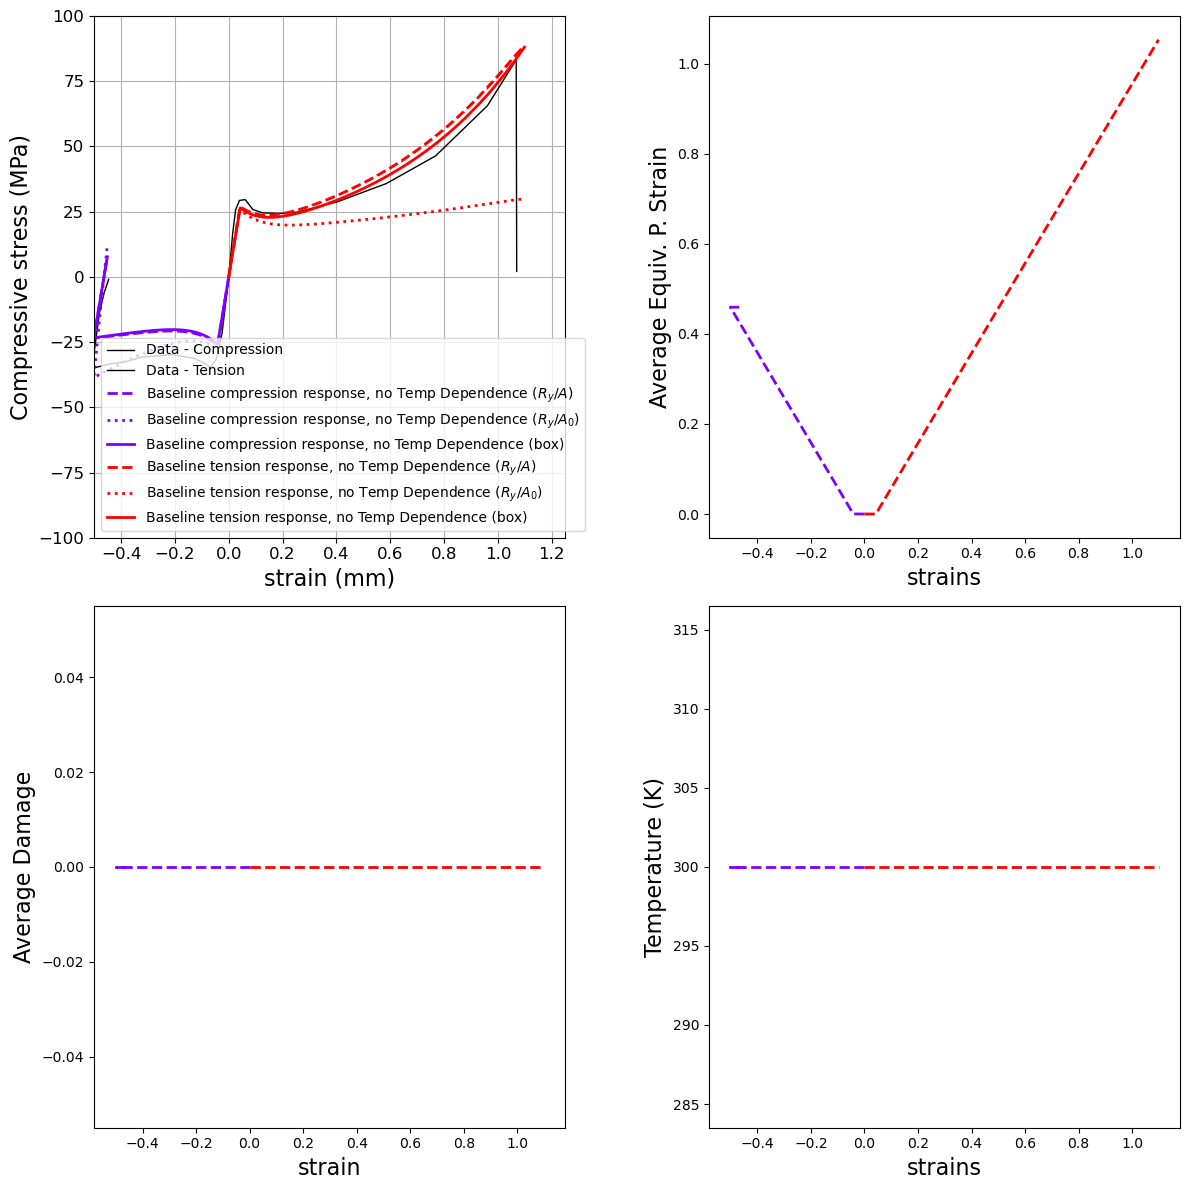
\includegraphics[width=0.42\linewidth]{../polymer/polymerCompressionTension.png}
\caption{Existing comparison assets in the source case directory.}
\end{figure}
\clearpage
\section*{polymer / polymerTension}
Validation case for Polymer validation.
\begin{figure}[H]\centering
\includegraphics[width=0.58\linewidth]{schematics/polymer\_\_polymerTension\_schematic.png}
\caption{Schematic for polymer\_\_polymerTension.}
\end{figure}
\textbf{Code features exercised.}
\begin{itemize}
\item reaction-history output
\item box-average history
\end{itemize}
\begin{figure}[H]\centering
\includegraphics[width=0.31\linewidth]{../polymer/output/polymer\_\_polymerTension/polymer\_\_polymerTension\_initial\_particleStrengthScale.png}
\includegraphics[width=0.31\linewidth]{../polymer/output/polymer\_\_polymerTension/polymer\_\_polymerTension\_final\_particleDamage.png}
\includegraphics[width=0.31\linewidth]{../polymer/output/polymer\_\_polymerTension/polymer\_\_polymerTension\_reaction.png}
\caption{Initial state, final state, and history/comparison plot for polymer\_\_polymerTension.}
\end{figure}
\paragraph{Reference or legacy comparison assets.}
\begin{figure}[H]\centering
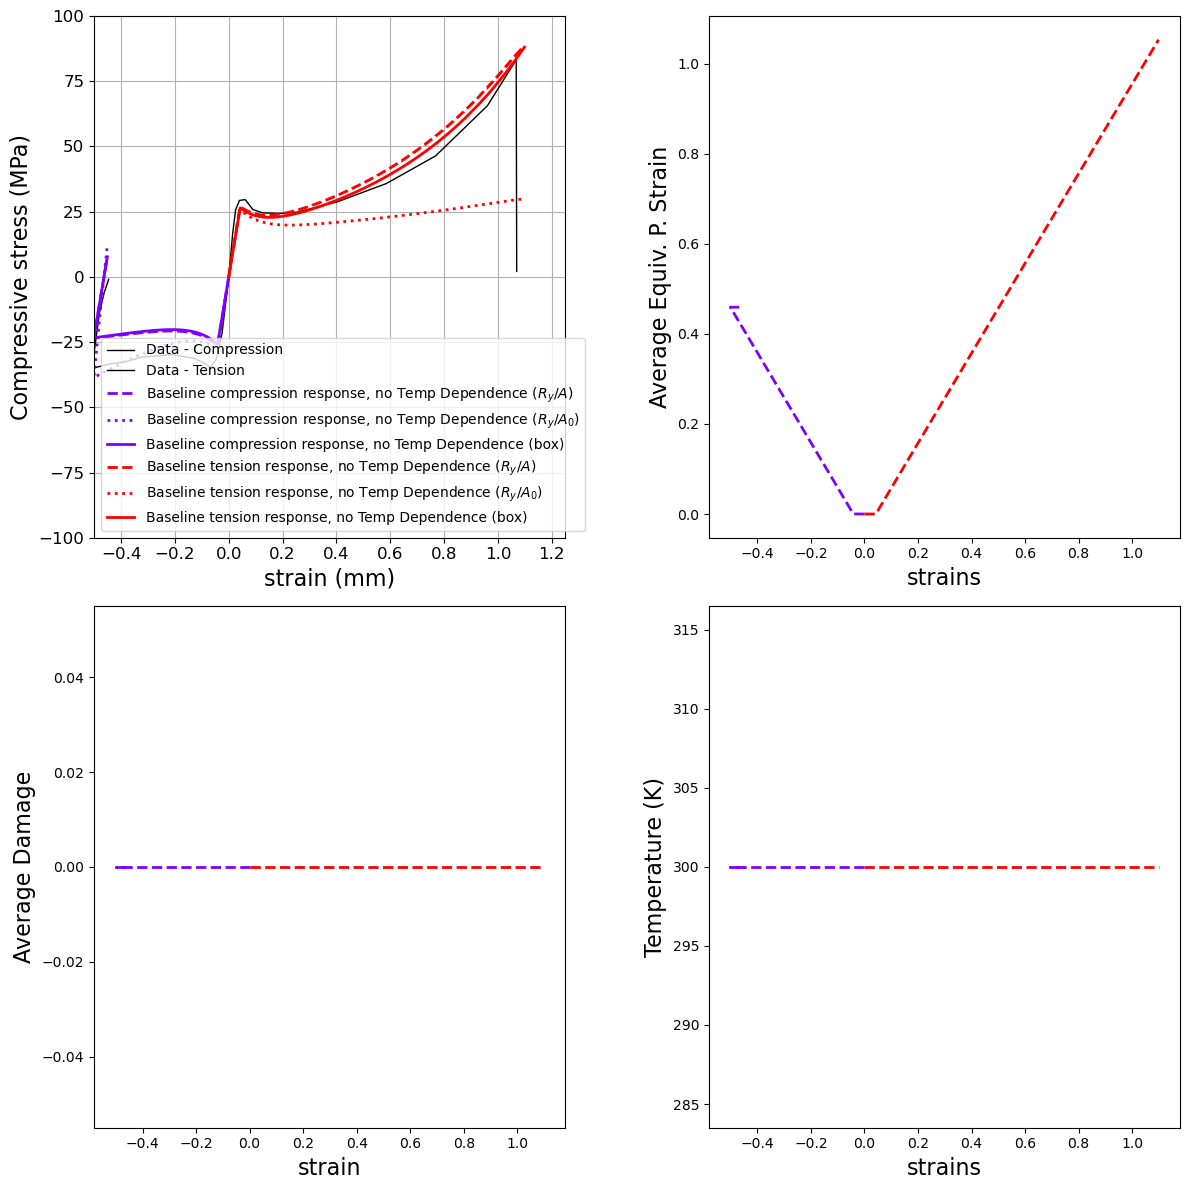
\includegraphics[width=0.42\linewidth]{../polymer/polymerCompressionTension.png}
\caption{Existing comparison assets in the source case directory.}
\end{figure}
\end{document}
